\part{Aspectos Gerais}

\chapter[Aspectos Gerais]{Aspectos Gerais}

Estas instruções apresentam um conjunto mínimo de exigências necessárias a 
uniformidade de apresentação do relatório de Trabalho de Conclusão de Curso 
da FGA. Estilo, concisão e clareza ficam inteiramente sob a 
responsabilidade do(s) aluno(s) autor(es) do relatório.

As disciplinas de Trabalho de Conclusão de Curso (TCC) 01 e Trabalho de 
Conclusão de Curso (TCC) 02 se desenvolvem de acordo com Regulamento 
próprio aprovado pelo Colegiado da FGA. Os alunos matriculados nessas 
disciplinas devem estar plenamente cientes de tal Regulamento. 

\section{Construção da Proposta}
\label{sec:constru_o_da_proposta}
A Rede Social About (RSA) tem o propósito de dar transparência às personalidades de seus usuários, permitindo com que todos
estes saibam sobre qualquer aspécto sobre qualquer outro usuário, dede que ambos tenham aceitado os
termos de consentimento pré estabelecidos.

Qualquer usuário pode criar abouts para seus amigos, que foram previamente aceitos. A fim de julgar
sobre a veracidade deste about, os demais amigos do usuário poderão votar sobre a veracidade,
julgando se é uma verdade ou uma mentira. Tanto o about escrito quando o voto são anônimos para todos os
usuários.

A proposta deste trabalho é desenvolver e aplicar uma instância do framework octalysis de gamificação na RSA, engajando e
motivando seus usuários a executarem determinadas tarefas que, serão discutidas posteriormente.

Os seguintes
passos serão estabelecidos para a execução proposta:

\begin{enumerate}
    \item Execução do teste piloto
    \item Survey para identificação das técnicas de gamificação
    \item Análise estatística das técnicas
    \item Construção do framework de gamificação
    \item Escolha do objeto de gamificação
    \item Implementação das técnicas no objeto de gamificação
\end{enumerate}

\subsection{Execução do Piloto}
\label{sub:execu_o_do_piloto}
A ideia sobre a rede social surgiu de uma simples ideia de um aluno de graduação. Desta forma, se até mesmo a
ideia era impalpável, algumas perguntas surgem sobre a gamificação desta, por exemple:

\begin{itemize}
    \item Como conseguir averiguar como traços de gamificação para ser aplicado?
    \item Como identificar quais são as motivações básicas que devem ser levadas em consideração?
    \item Para atingir tais motivações, quais são as técnicas que devem ser adotas?
\end{itemize}

Para responder essas perguntas, que irão servir de insumo para o direcionamento dos pilares da gamificação, será elaborado um projeto pilotor, tal qual terá algumas funcionalidades básicas da RSA, sem levar em consideração requisitos não funcionais como: segurança, usabilidade, performance e padrões de design.

O objetivo é proporcionar aos usuários um cenário similar, quanto a funcionalidade, ao que estes irão utilizar
na RSA, a fim de identificar quais as técnicas de gamificação são mais presentes.

Para desenvolver e aplicar este piloto, será necessário executar um procedimento com os seguintes passos:
% definir tecnologia,
% desenvolver a solução, virá-la para produção, aplicar marketing da solução para um público reduzido, manter solução, finalizar solução.

\begin{itemize}
    \item Definir tecnologia
    \item Desenvolver solução
    \item Virá-la para produção
    \item Aplicar marketing da solução para um público reduzido
    \item Manter solução
    \item Finalizar solução
\end{itemize}

Estes pontos necessários para que a implementação da solução do projeto piloto serão detalhados a seguir:

\subsubsection{Definir Tecnologia}
\label{sub:definir_tecnologia}
Como o desenvolvimento da solução para o projeto piloto não necessita conter interfaces com design bem elaborado;
usabilidade, baseado em user experience, elavada; dentre outras necessidades não funcionais. Os critérios levados em
consideração para a sua construção foram os seguintes:

\begin{itemize}
    \item Desenvolvimento rápido: por se tratar de uma simples solução, temporária, o tempo de implementação deveria
        ser curto, levantando o requisito de utilizar um framework de alta produtividade.
    \item Padrões de Design simples: por se tratar de uma aplicação extremamente funcional, tal que o usuário não irá
        utilizá-la por muito tempo, não há a necessidade de fortes esforços e grande elaboração dos padrões de
        User Experience.
    \item Escalabilidade baixa: como se trata de um público pequeno, para poucos usuários simultâneos, em torno de duzentos
        acessos diários, o framework pode ser de baixo desenpenho, facilitanto assim a sua escolha.
    \item Os usuários não carecem de executar cadastros e logins: para o escopo do piloto, cada usuário não necessitará
        fazer registros e logins no site. A política de gerenciamento dos votos será feita mediante armazenamento dos
        IP's utilizados durante o acesso, fazendo com que cada IP possa votar apenas uma vez dentro de um determinado
        intervalo de tempo.
    \item Suporte para questionários: como o piloto se trata de quistionários baseados em perguntas, há a necessidade que o framework
        escolhido conceda suporte para criação de perguntas, possibilidade de votação, vizualização e contagem dos votos
        separados por perguntas.
    \item Facilidade de implantação: como se trata de um site web bem rápido, há a necessidade de que este seja de fácil e rápida
        implantação, possibilitando que rápidamente seja colocado em produção. Dessa forma, o framework escohido também carece
        de propiciar suporte para esta feature.
\end{itemize}

Dados os requisitos acima, irá se iniciar um processo de busca por ferramentas e frameworks que possibilitem a implentação do site
web que os contemple. Para a avaliação, as ferramentas levantadas, que serão até cinco, irão ser submetidas à uma tabela que contempla
os requisitos básicos necessários. Cada item da tabela poderá ser julgado de um a cinco, sendo que a nota 1 diz que a ferramenta não nada
desta funcionalidade, já a nota 5 diz que esta contém totalemente esta funcionalidade. Assim, os valores intermediários: 2, 3 e 4 representam
que possuem o requisito parcialmente, de acordo com a nota.

% \usepackage{booktabs}
\begin{table}[]
    \centering
    \begin{tabular}{@{}llllll@{}}
        \toprule
        \textbf{}                                                  & \textbf{Tool A}       & \textbf{Tool B}       & \textbf{Tool C}       & \textbf{Tool D}       & \textbf{Tool E}       \\ \midrule
        \multicolumn{1}{|l|}{\textbf{Desenvolvimento Rápido}}      & \multicolumn{1}{l|}{} & \multicolumn{1}{l|}{} & \multicolumn{1}{l|}{} & \multicolumn{1}{l|}{} & \multicolumn{1}{l|}{} \\ \midrule
        \multicolumn{1}{|l|}{\textbf{Padrões de Design Simpels}}   & \multicolumn{1}{l|}{} & \multicolumn{1}{l|}{} & \multicolumn{1}{l|}{} & \multicolumn{1}{l|}{} & \multicolumn{1}{l|}{} \\ \midrule
        \multicolumn{1}{|l|}{\textbf{Sem Autenticação}}            & \multicolumn{1}{l|}{} & \multicolumn{1}{l|}{} & \multicolumn{1}{l|}{} & \multicolumn{1}{l|}{} & \multicolumn{1}{l|}{} \\ \midrule
        \multicolumn{1}{|l|}{\textbf{Baixa Escalabilidade}}        & \multicolumn{1}{l|}{} & \multicolumn{1}{l|}{} & \multicolumn{1}{l|}{} & \multicolumn{1}{l|}{} & \multicolumn{1}{l|}{} \\ \midrule
        \multicolumn{1}{|l|}{\textbf{Suporte para Questionário}}   & \multicolumn{1}{l|}{} & \multicolumn{1}{l|}{} & \multicolumn{1}{l|}{} & \multicolumn{1}{l|}{} & \multicolumn{1}{l|}{} \\ \midrule
        \multicolumn{1}{|l|}{\textbf{Facilidade de Implementação}} & \multicolumn{1}{l|}{} & \multicolumn{1}{l|}{} & \multicolumn{1}{l|}{} & \multicolumn{1}{l|}{} & \multicolumn{1}{l|}{} \\ \midrule
                                                                   &                       &                       &                       &                       &                       \\ \midrule
                                                                   \multicolumn{1}{|l|}{\textbf{Total}}                       & \multicolumn{1}{l|}{} & \multicolumn{1}{l|}{} & \multicolumn{1}{l|}{} & \multicolumn{1}{l|}{} & \multicolumn{1}{l|}{} \\ \bottomrule
    \end{tabular}
    \caption{Avaliação dos Frameworks}
    \label{my-label}
\end{table}

Cada ferramenta, no final da avaliação, terá uma nota entre 6 e 30, que será disposta na linha 'Total'. Assim, a ferramenta que possuir a maior nota será escolhida para a execução do projeto piloto.

\subsubsection{Desenvolver Solução}
\label{sub:definir_tecnologia}

Dada a ferramenta escolhida, faz-se necessário que esta seja analizada em termos técnicos. Será necessário analisar e seguir alguns pontos, que
serão descritos abaixo para que a solução seja implementada com sucesso:

\begin{enumerate}
    \item Escolher versão do framework que será utilizado;
    \item Executar download do framework para o laboratório local, que terá os testes executados;
    \item Executar instalação da ferramenta em um laboratório local, que será utilizado como ambiente de
        desenvolvimento da aplicação;
    \item Definir qual template será utilizado para a página home do site, layout da aplicação e menu principal;
    \item Executar o download do plugin de execução de questionários na página principal do framework que será escolhido;
    \item Instalar na aplicação o plugin para a criação, manutenção e vizualização dos questionários;
    \item Configurar plugin de questionários para armazenar as perguntas e os índices de votação de cada pergunta em persistência;
        Para que posteriormente seja possível executar a análise de todos os dados coletados;
    \item Executar a criação de um questionário a fim de homologar a solução desenvolvida para os pré-requisitos estabelecidos. 
    \item Executar a integração da questão criada para homologação no layout da home da aplicação;
    \item Executar o gerenciamento de configuração de software para que o código fonte seja armazenado. Este será posteriormente
        capturado para executar a aplicação no servidor de produção;
\end{enumerate}

Com todos esses passos executados, a solução está operando de acordo como o esperado para recolher os dados básicos propostos anteriormente.
Assim, esta está preparada para ser disposta em produção em um servidor e disponibilizá-la para o público geral. Na próxima sessão serão
detalhados os passos para ter a aplicação em produção.

\subsubsection{Virá-la para a Produção}
\label{sub:definir_tecnologia}
Para que qualquer pessoa com acesso à internet possa conseguir ter acesso à aplicação desenvolvida, faz-se necessário que
o site hospedado esteja em um servidor com um IP externo válido. Para melhor utilização da plataforma, será necessário adquirir um domínio
que faça o apontamento para o IP do servidor adquirido. 

Os passos necessários para virar o servidor de produção serão descritos nos itens seguintes:

\begin{enumerate}
    \item Avaliar qual será o provedor de máquinas virtuais será utilizado;
    \item Adquirir uma máquina virtual com IP externo. Este deve conter o mínimo possível de capacidade de processamento e
        disponibilidade de memória RAM para que seja possível suportar a hospedagem da solução;
    \item Adquirir um domínio em um servidor DNS do server .com.br para apontamento do IP externo;
    \item Configurar o domínio DNS adquirido para que este execute o apontamento do IP do servidor que será utilizado;
    \item Executar instalação de um servidor de páginas HTTP no servidor;
    \item Executar a instalação de uma base de dados para armazenamento das informações obtidas;
    \item Recuperar o código fonte utilizado no ambiente de desenvolvimento para o servidor. Este será devidamente
        instalado e recuperado assim como foi feito anteriormente;
    \item Executar as configurações do framework para que este opere corretamente utilizando um servidor externo;
    \item Executar a criação novamente de uma questão para que seja possível homologar o ambiente de produção.
\end{enumerate}

Estes passos vão assegurar que o servidor seja configurado corretamente e que esteja disponível para acesso externo para
todos os usuários que vão o sistema.

Com os procedimentos necessários para que o projeto piloto esteja acessível pelos usuários, já será possível executar o marketing
para divulgar a algumas pessoas a aplicação. Os passos para o marketing serão descritos no próximo sub tópico.

\subsubsection{Aplicar Marketin do projeto piloto}
\label{sub:definir_tecnologia}
Como se faz necessário que haja usuários utilizando o protótipo para recolher os dados, é fundamental que o propósito
e o protótipo sejam divulgados para o público externo que irá utilizá-lo. 

A proposta de marketing seguirá algumas diretivas que serão apresentadas a seguir:

\begin{enumerate}
    \item O público alvo foi definido para que este pudesse ser atingido facilmente. Como estamos tratando de um
        projeto de desenvolvendo universitário, este meio pode ser facilmente almejado em pouco tempo. Isto se
        deve ao volume de alunos existentes no campus com disponibilidade para testar novos projetos e ideias.
        Desta maneira, o público alvo serão os universitários da UnB unidade Gama - Distrito federal(UnB-FGA).
    \item Como estamos tratando de um projeto piloto que carece da presença de usuários a utilizando, alguns
        pontos são extremamente importante para que o público alvo definido seja atingido. Assim, o meio de
        distribuição do protótipo deve conter os seguintes pontos:
        \begin{itemize}
            \item Ser possível compartilhar os links publicados no protótipo;
            \item Novas enquentes devem chegar rapidamente ao público alvo;
            \item Novas enquentes devem ser dispostas em um meio que esteja disponível para todos os
                alunos do campus FGA.
        \end{itemize}
    \item Existem vários meios possíveis para alcançar o público alvo, por exemplo:
        \begin{itemize}
            \item Contato direto verbal;
            \item Cartazes e planfetos no campus;
            \item Listas de emails;
            \item Sites de fóruns da UnB;
            \item Sites de devulgação;
            \item Grupos e páginas do facebook.
        \end{itemize}
    \item Desta forma, será escolhido o meio de comunicação que atenda de melhor maneira os pré-requisitos descritos acima. Para que
        seja possível compartilhar links, demonstrar rapidamente novas enquente e com o maior número de estudantes, o melhor meio de
        comunicação é a utilização do facebook. Utilizando o facebook, é possível utilizar o grupo da faculdade, que contém vários alunos,
        levantando em consideração que os links podem ser compartilhados por lá. Dessa forma, toda a apresentação do protótipo será executada
        via grupo da faculdade no facebook;
    \item Todas as novas enquetes serão apresentadas no grupo e compartilhadas também no grupo do facebook do campus da faculdade.
\end{enumerate}

Assim, todas as novas enquetes irão seguir os padrões estabelecidos nestas diretrízes de regras de marketing. Isto irá assegurar que
o público alvo escolhido seja aumejado.


\subsubsection{Manter a Solução}
\label{sub:definir_tecnologia}
Após a construção estabelecida e disponível para que os usuários a utilizem, já é possível aplicar novos questionários, fazendo uso do plano de marketing.
Esta etapa consistirá em criar um sistema em que os próprios usuários vão ceder as novas informações para novos questionários. Estes questionários 
terão as informações coletadas e futuramente utilizadas.

Primeiramente, será criada uma segunda página para o site. Esta página será responsável por conter uma enquente com a seguinte pergunta:

 \begin{quote}
     "Qual deve ser a próxima enquete do site?"
 \end{quote}

As perguntas dispostas serão analisadas e as que foram consideradas de bom gosto, serão utilizadas. A cada dia, uma nova questão será aprensentada
para a enquente. Essa nova enquente será publicada e compartilhada. Após 48 horas, esta será dada como finalizada e o resutaldo será apresentado
para o público. 

Este ciclo será mantido por duas semanas, possibilitando com que sejam elaborados materias suficientes para recolher os indicadores que necessitamos 
das técnicas de gamificação da rede social.
\subsubsection{Finalizar a Solução}
\label{sub:definir_tecnologia}

Após duas semanas de uso da solução proposta, os dados serão recolhidos e o servidor será desligado para evitar gastos. O domínio continuará em operação
por mais um ano, porém, não apontará para um endereço de IP válido, pois, o servidor que conterá o endereço externo não estará mais em operação.

Este será o tempo necessário para implantar e recolher todas as informações propostas para o uso da solução de projeto piloto.

\subsection{Levantamento das Técnicas de Gamificação}
\label{sub:survey_para_t_cnicas_de_gamifica_o}
Será executado um levantamento com alguns usuários aleatoriamente escolhidos dentre os que interagiram com o piloto.
O objetivo do levantamento é identificar quais são as técnicas de gamificação mais presentes no piloto executado.

O levantamento será executado em duas etapas. A primeira se trata de conseguir entender o que os usuários entendem e pensam sobre o objetivo
principal que o projeto piloto terá a intenção de retratar. A segunda parte consistirá na elaboração de um survey com opções de valores entre 1 e 5,
listando todas as técnicas de gamificação existentes no octalysis.

Os procedimentos sobre como serão elaboradas as duas próximas etapas serão descritas nas duas sessões seguintes. 

\subsubsection{Características Projeto do Piloto}
\label{sub:caracter_sticas_projeto_do_piloto}
Com a intenção de compreender a visão que os usuários irão ter do projeto, bem como entender onde podem ser trabalhadas suas motivações básicas,
serão levantadas as suas características.

Este processo será elaborado fazendo com que os usuários respondam três perguntas abertas. As perguntas são as seguintes:

\begin{quotation}
    Questão 01: Na sua opinião, o que este site representava?
\end{quotation}

\begin{quotation}
    Questão 02: O que você acredita que motivava e levava as pessoas a utilizarem o site?
\end{quotation}

\begin{quotation}
    Questão 03: E quanto ao contrário, o que você acredita que levava as pessoas a se desmotivarem e a não
    utilizar mais o site?
\end{quotation}

Estas questões serão feitas a alguns usuários do sistema individualmente. As suas respostas serão gravadas para futuras análises.
Além disso, as respostas serão transcrevidas para o relatório.

\subsection{Survey das Técnicas}
\label{sub:survey_das_t_cnicas}
Com o intuito de analisar as motivações básicas em questão de quanto é necessário para que esta se enquadre no projeto
de gamificação, iremos aplicar um survey com várias técnias oriundas do octalysis. Essas técnicas serão submetidas à alguns
usuários do protótipo para avaliarem o quanto aquela técnica se enquadra dentro do escopo. Essas técnicas serão julgadas de 1
a 5. Sendo que da mesma forma para que a avaliação das ferramentas e frameworks, serão atribuídas às técnicas com
muita presença a nota cinco e para as técnicas com pouca presença a nota um. Sendo assim, os valores intermediários
também representam presenças intermediárias destes, na mesma proporção.

As técnicas que serão aplicadas já foram selecionadas no framework. Elas serão as seguintes listadas a seguir:

\begin{multicols}{2}
    \begin{enumerate}
        \item Narrative
        \item Beginner's Luck
        \item Free Lunch
        \item Elitism
        \item Humanity Hero
        \item Higher Meaning
        \item Destiny Child
        \item Status Points/Points
        \item Achievement Symbols/ Badges
        \item Leaderboards
        \item Progress Bar
        \item Glowing Choice
        \item Desert Oasis
        \item The Rockstar Effect
        \item Fixed Actions Rewards/Earned Lunch
        \item Quest List
        \item High Five
        \item Crowning
        \item LevelUp Symphony
        \item Aura Effect
        \item Step-by-Step Tutorial
        \item Boss Fight
        \item Evergreen Mechanics
        \item General's Carrot
        \item Real-Time Control
        \item Chain Combos
        \item Instant Feedback
        \item Blank Fills
        \item Voluntary Autonomy
        \item Choice Perception/Poison Picker
        \item Plant Picker/ Meaningful Choices
        \item Milestone Unlock
        \item Boosters
        \item Virtual Goods
        \item Build from Scratch
        \item Collection Set
        \item Exchangeable Points
        \item Monitor Attachment
        \item The Alfred Effect
        \item Mentorship
        \item Bragbuttons
        \item Trophyshelves
        \item Group Quest
        \item Social Treasures
        \item Social Proud
        \item Conformy Anchor
        \item Water Cooler
        \item Friending
        \item SeeSaw Bump
        \item Touting
        \item Bragging
        \item Thank-You Economy
        \item Dangling
        \item Ancored Juxtaposition
        \item Prize Pacing
        \item Options Pacing
        \item Patient Feedback
        \item Count Down
        \item Throttles
        \item Moats
        \item TortureBreak
        \item Envolved UI
        \item Glowing Choice
        \item Mystery Boxes/ Random Rewards
        \item Easter Eggs
        \item Sudden Rewards
        \item Visual Storytelling
        \item Obvious Wonder
        \item Rolling Rewards
        \item Mischief Puzzle
        \item Oracle Effect
        \item Lottery (Rolling Rewards)
        \item Mini Quests
        \item Countdown Timer
        \item Status Quo Sloth
        \item FOMO Ponch
        \item Sunk-Cost Tragedy
        \item Lost Progress
        \item Scarlett Letter
        \item Visual Grave
    \end{enumerate}
\end{multicols}

Agora, como será mapeado o quanto cada motivação básica está presente no projeto piloto? Simples, como dito antes,
cada técnica pertence a uma motivação básica. Desta forma, será simples mapear o quanto cada técnica estará presente.

Como citado anteriormente, existem oito motivações básicas, e cada uma agloba um conjunto de técnicas. As oito motivações básicas são as seguintes:

\begin{enumerate}
    \item Significado Épico \& Chamado
    \item Desenvolvimento \& Realização
    \item Empoderamento \& Feedback
    \item Propriedade \& Posse
    \item Influência Social \& Pertencimento
    \item Escassez \& Impaciência
    \item Imprevisibilidade \& Curiosidade
    \item Perda \& Rejeição
\end{enumerate}

Como se dará o cálculo para verificar a presença de uma motivação básica na aplicação?

Uma média simples poderia atender a identificação das motivações básicas, dada pela seguinte fórmula: \\ \\


$ MediaCadaMotivacao = \frac{PontosTotais}{QuantidadeMotivacoes} $

$ PontosMotivacao = \frac{MediaCadaMotivacao}{\sum PontosCadaMotivacao} $


$Onde:
\\ \\$
QuantidadeMotivacoes = 8
\\ PontosTotais = Somatório do máximo de pontos possíveis dentro da votação.
\\ MediaCadaMotivacao = Média aritmética de quantos pontos máximos cada motivação pode conter.
\\ PontosCadaMotivacao = Quantidade de pontos obtida pela votação.
\\ PontosMotivacao = Percentagem de pontos que a motivação possui. \\ \\


 Porém, observamos que esta média se torna injusta com algumas motivações e compromete o resultado final.
Isso ocorre pois  algumas motivações básicas possuem mais técnicas do que outras, fazendo com que
as que possuem poucas técnicas consigam somar uma baixa quantidade de pontos para aplicar no percentual final perante
à média de todas as outras.

Desta forma, para que as médias sejam relativas dentro de cada motivação, foi decidido que as médias serião avaliadas dentro da
própria motivação. Desta forma, será executado um cálculo para cada motivação, onde o objetivo é identificar quais são
as suas respectivas notas máximas possíveis. Logo após, serão executadas contagens dos pontos de cada motivação quanto à votação.
Esses dados serão utilizados para resultar a média, dividido os pontos totais pelos pontos de votação. 

Desta forma, a equação para calcular a média de cada pontuação se dará como o descrito a seguir:

$PontosMotivação = \frac{\sum PontoMáximo}{PontosCadaMotivacao}\\Onde:$

PontoMáximo = Quantidade máxima de ponto dentro de cada técnica.


Desta forma, teremos total certeza que cada motivação básica terá a sua nota justa perante todas as demais e não será prejudicada
pela sua quantidade. Assim, será possível aplicar estas fórmulas para obter os dados corretamente.

Através dos dados utilizando as médias, será possível desenhar um primeiro esboço do framework, identificando quais são as motivações
básicas que os usuários mais conseguem ver na aplicação. 

O criador do Octalasys implementou e disponibilzou uma ferramenta para executar desenhos da forma como o framework está implementado
de acordo com o quão presentes são algumas técnicas. Esta aplicação pode ser vista no site oficial do framework.

Abaixo está ilustrada um exemplo da ilustração do frameworuma ferramenta para executar desenhos da forma como o framework está implementado
de acordo com o quão presentes são algumas técnicas. Esta aplicação pode ser vista no site oficial do framework.

A Figura \ref{fig:exoctalysis} está ilustrada um exemplo da ilustração do framework.

 \begin{figure}[h]
     \centering

     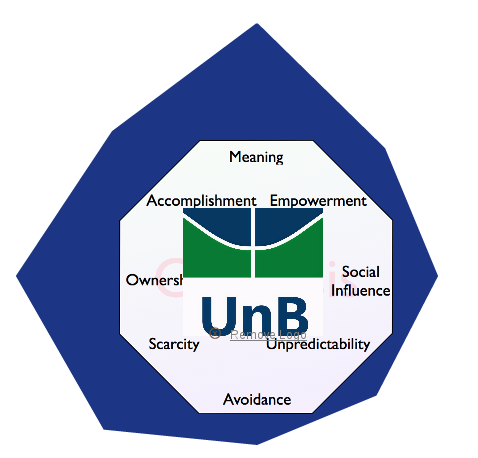
\includegraphics[width=300px, scale=1]{figuras/exoctalysis}
     \caption{Exemplo do framework octalysis}

     \label{fig:exoctalysis}
 \end{figure}


Nela, podemos observar que cada motivação básica possui algum valor atribuído, e isto representa o quanto desta existe no escopo que
está sendo testado. O percentual de quanto cada motivação básica é importante estará representado na Tabela \ref{exmotivacao}:

% Please add the following required packages to your document preamble:
% \usepackage{booktabs}
\begin{table}[]
    \centering
    \caption{Índice de presença das motivações: exemplo}
    \label{exmotivacao}
    \begin{tabular}{@{}|c|c|@{}}
        \toprule
        \textbf{Motivação Básica}          & \textbf{\begin{tabular}[c]{@{}c@{}}Porcentagem\\ (\%)\end{tabular}} \\ \midrule
            Significado Épico \& Chamado       & 100                                                                 \\ \midrule
        Desenvolvimento \& Realização      & 60                                                                  \\ \midrule
        Empoderamento \& Feedback          & 40                                                                  \\ \midrule
        Propriedade \& Posse               & 90                                                                  \\ \midrule
        Influência Social \& Pertencimento & 40                                                                  \\ \midrule
        Escassez \& Impaciência            & 70                                                                  \\ \midrule
        Imprevisibilidade \& Curiosidade   & 30                                                                  \\ \midrule
        Perda \& Rejeição                  & 30                                                                  \\ \bottomrule
    \end{tabular}
\end{table}


Desta forma, será necessário gerar este framework para as médias básicas retiradas do projeto piloto e desenhar esta tabela com os
seus respectivos valores, que, provavelmente não serão tão precisos quanto aos que foram utilizados no exêmplo.

A figura do framework e a tabela que serão gerados permitiram à quem irá analisar e avaliar o framework ter uma interpretação
visual dos níveis de motivações básicas no sistema e como elas se relacionam.

Utilizando esses cálculos básicos de média, e com as notas da votação, será possível realizar cálculos estatíticos para a construção
das análises a respeito das técnicas de gamificação.



\subsection{Análise Estatística das Técnicas}
\label{sub:an_lise_estat_stica_das_t_cnicas}
A partir da massa de dados obtida com o survey, serão executadas análises estatícas a fim de identificar correlações
entre as regras e permitir que seja possível entender quais são as técnicas mais presentes e o mais importante, como
estas se relacionam entre si, para que seja possível fazer aferições sobre qual técnica está ligada a qual outra.

Para realizar estas análises estatíticas, são necessários alguns passos que serão justificados a seguir:

\begin{enumerate}
    \item Definir ferramenta para realização das análises estatícas: a massa de dados é consideravelmente grande, devido 
        a grande quantidade de técnicas valoradas. Assim, utilizar planilhas do excel ou simplesmentes cálculos diretos
        podem dificutar a utilização, realização e armazenamento de cálculos. Dessa forma, será adotada uma linguagem
        de script utilizada para análises estatísticas;
    \item Importação dos dados oriundos do survey;
    \item Parser dos dados importados;
    \item Calcular o alpha de cronbach, para averiguar e conseguir estabelecer a confiabilidade do survey analisado;
    \item Para identificar as relações entre as técnicas, primeiramente, será utilizada a correlação de pearson;
    \item Sumarizar das correlações de pearson;
    \item Transformar dos dados da matrix em trasações;
    \item Calcular o algoritimo apriori, para identificar quais técnicas irão ser diretamente ligadas as outras.
\end{enumerate}

Desta forma, nas sessões seguintes, serão detalhados os passos que foram agora pouco pontuados.

\subsubsection{Ferramenta para Estatística}
\label{sub:ferramenta_para_estat_stica}
Como foi dito agora pouco, para o escomo que estamos trabalhando, apenas uma planilha excel não será suficiente
para a manutenção, processamento e armazenamento dos dados obtidos. Dessa forma, será  necessário um processo
para levantamento da ferramenta que será utilizada.

Nosso escopo irá carecer de alguns requisitos que serão descritos a seguir:

\begin{itemize}
    \item Suporte à importação de dados em arquivos ods, xls, csv;
    \item Suporte à exportação de dados em arquivos ods, xls, csv;
    \item Suporte a algorítimo de cálculo da correlação de peason;
    \item Suporte a algorítimo de cálculo do alpha de cronbach;
    \item Suporte a algorítimo de relações apriori;
    \item Possibilidade de manupulação de matrizes;
    \item Possibilidade para executar os memos passos consecutivas vezes;
    \item Flexibilidade para manutenção.
\end{itemize}

Para tanto, serão levantadas três ferramentas de análise estatística. Estas serão submetidas a uma ficha de avaliação.
Cada requisito terá uma nota de um a cinco para itens que podem ser valorados, sendo que a ferramenta que melhor pontuar será a escolhida.

A Tabela \ref{avalicaoferramentaestatistica} será utilizada para a avaliação de atributos, sendo que serão
pontuados entre um e cinco. Sendo que se não possuir o atributo, será adotada a nota 1, e caso possua, será
atribuída a nota cinco.
% Please add the following required packages to your document preamble:
% \usepackage{booktabs}
\begin{table}[]
    \centering
    \caption{Avaliação - Ferramenta Estatística}
    \label{my-label}
    \begin{tabular}{@{}llll@{}}
        \toprule
        \multicolumn{1}{|l|}{}                                       & \multicolumn{1}{l|}{\textbf{Ferramenta A}} & \multicolumn{1}{l|}{\textbf{Ferramenta B}} & \multicolumn{1}{l|}{\textbf{Ferramenta C}} \\ \midrule
        \multicolumn{1}{|l|}{\textbf{Manipulação de matrizes}}       & \multicolumn{1}{l|}{}                      & \multicolumn{1}{l|}{}                      & \multicolumn{1}{l|}{}                      \\ \midrule
        \multicolumn{1}{|l|}{\textbf{Comandos repetidas vezes}}      & \multicolumn{1}{l|}{}                      & \multicolumn{1}{l|}{}                      & \multicolumn{1}{l|}{}                      \\ \midrule
        \multicolumn{1}{|l|}{\textbf{Flexibilidade de manutenção}}   & \multicolumn{1}{l|}{}                      & \multicolumn{1}{l|}{}                      & \multicolumn{1}{l|}{}                      \\ \midrule
        \multicolumn{1}{|l|}{\textbf{Importação CSV}}                & \multicolumn{1}{l|}{}                      & \multicolumn{1}{l|}{}                      & \multicolumn{1}{l|}{}                      \\ \midrule
        \multicolumn{1}{|l|}{\textbf{Importação XLS}}                & \multicolumn{1}{l|}{}                      & \multicolumn{1}{l|}{}                      & \multicolumn{1}{l|}{}                      \\ \midrule
        \multicolumn{1}{|l|}{\textbf{Importação ODS}}                & \multicolumn{1}{l|}{}                      & \multicolumn{1}{l|}{}                      & \multicolumn{1}{l|}{}                      \\ \midrule
        \multicolumn{1}{|l|}{\textbf{Exportação CSV}}                & \multicolumn{1}{l|}{}                      & \multicolumn{1}{l|}{}                      & \multicolumn{1}{l|}{}                      \\ \midrule
        \multicolumn{1}{|l|}{\textbf{Exportação XLS}}                & \multicolumn{1}{l|}{}                      & \multicolumn{1}{l|}{}                      & \multicolumn{1}{l|}{}                      \\ \midrule
        \multicolumn{1}{|l|}{\textbf{Exportação ODS}}                & \multicolumn{1}{l|}{}                      & \multicolumn{1}{l|}{}                      & \multicolumn{1}{l|}{}                      \\ \midrule
        \multicolumn{1}{|l|}{\textbf{Alpha de Croncach}}             & \multicolumn{1}{l|}{}                      & \multicolumn{1}{l|}{}                      & \multicolumn{1}{l|}{}                      \\ \midrule
        \multicolumn{1}{|l|}{\textbf{Algorítimo Apriori}}            & \multicolumn{1}{l|}{}                      & \multicolumn{1}{l|}{}                      & \multicolumn{1}{l|}{}                      \\ \midrule
        \multicolumn{1}{|l|}{\textbf{Transformação para transações}} & \multicolumn{1}{l|}{}                      & \multicolumn{1}{l|}{}                      & \multicolumn{1}{l|}{}                      \\ \midrule
        \multicolumn{1}{|l|}{\textbf{Correlação de Pearson}}         & \multicolumn{1}{l|}{}                      & \multicolumn{1}{l|}{}                      & \multicolumn{1}{l|}{}                      \\ \midrule
                                                             &                                            &                                            &                                            \\ \midrule
        \multicolumn{1}{|l|}{Total}                                  & \multicolumn{1}{l|}{}                      & \multicolumn{1}{l|}{}                      & \multicolumn{1}{l|}{}                      \\ \bottomrule
    \end{tabular}
\end{table}

Após totalizar as pontuações totais das ferramentas, está será selecionada e preparada para a utilização e execução dos cálculos.

Os passos necessários para que a ferramenta esteja apta para o uso das análises dos scripts serão detalhados abaixo:

\begin{enumerate}
    \item Download da ferramenta através do site oficial;
    \item Instalção da ferramenta no ambiente local que será desenvolvido o código;
    \item Adaptação da IDE utilizada pelo desenvolvedor para que seja compatível à ferramenta escolhida.
\end{enumerate}

Adotados estes passos, a ferramenta estará pronta para receber a aplicação e executar todos os scripts, cálculos que serão
necessários.

\subsubsection{Importação dos Dados}
\label{sub:importa_o_dos_dados}
De antemão, já se tem informação que  os dados do survey serão recolhidos e armazenados em uma planilha de algum dos seguintes tipos:

\begin{itemize}
    \item Planilhas Excel do Word - XLS;
    \item Planilhas Calc do Libre - ODS;
    \item Planilhas Separada por Vírbula - CSV.
\end{itemize}

Assim, já sabemos que será necessário executar a importação destes dados. Como a ferramenta escolhida tem como pré-requisitos
essa feature, esta não será uma preocupação, pois sabemos que ela se encarregará da execução deste ponto. Porém, para realizar
a importação corretamente, serão necessários alguns passos:

\begin{enumerate}
    \item Executar a instalação dos pacotes necessários para ler os tipos de arquivos citados anteriormente;
    \item Carregar o pacote a ser utilizado para a importação que ocorrerá;
    \item Executar a importação dos dados através do arquivo de armazenamento da planilha;
    \item Armazenar em memória RAM os dados importados.
\end{enumerate}

\subsubsection{Alpha de Cronbach}
\label{sub:alpha_de_cronbach}
Como é possível identificar se os resultados do nosso survey está confiável?

É possível que alguma variável esteja diminuindo o índice de confiabilidade do questionário?

Essas perguntas são facilmente respondidas pelo alpha de cronbach. Este irá identificar entre as regras quais possuem
um elevado nível de correlação entre si, aferindo através de suas fórmulas qual a confiabilidade do que foi obtido.

O Alpha retorna valores entre um e zero, onde os valeres aceitáveis estão na faixa de 0.6 e 0.9.

Também é possível que o Alpha nos retorne qual seria o novo índice de confiabilidade caso um item específico seja removido.
Isso permite com que isolando algumas partes do questionário, a confiabilidade melhore.

Alguns passos são necessários para calcular o Alpha. Estes procedimentos serão descritos a seguir:

\begin{enumerate}
    \item Instalar o módulo para o Alpha de Cronbach;
    \item Carregar o módulo para o Alpha de Cronbach;
    \item Remover todos os campos dos dados com valores nulos;
    \item Remover todos os campos da tabela com números diferentes de [1, 2, 3, 4, 5];
    \item Habilitar a aplicação para apresentar os cabeçalhos das variáveis;
    \item Executar a função que executa o cálculo do Alpha;
    \item Averiguar se o resultado do índice está dentro dos padrões aceitáveis para o Alpha de Cronbach;
    \item Caso o valor esteja fora dos valores permitidos, desabilite a variável que mais está tendo impácto negativo no indicador,
        ou seja, remova aquela com o índice mais distante de 0.6 e 0.9, e volte para o item 6.
    \item Caso o valor esteja satisfatório, passe a considerar para os próximos cálculos apenas as variáveis que foram
        escolhidas com alta confiabilidade;
    \item Para que seja possível utilizar um tracking dos resultados posteriormente, estes devem ser exportados para uma planilha.
        Esta planilha deve ser de algum dos tipos estipulados para a escolha da ferramenta, de modo a garantir que está terá suporte
        para efetuar uma dada atividade.
    \item Para melhor organmização do projeto, deverá ser criada uma pasta que armazenará todos os resultados gerados pelo cálculo do Alpha
        de Cronbach.
\end{enumerate}

Agora que é possível ter confiablidade nos dados, de acordo com os resultados apresentados pelos algoritimos utilizados, será
possível
utilizar outros cálculos para aferir a correlação entre as técnicas.

O primeiro ponto requerido é, a partir dos dados tratados, aplicar a correlação de pearson. Esta correlação irá ilustrar
quanto cada técnica se assemelha com outra. Esta é representada em uma matriz, contendo em cada célula, um valor que varia entre um
e zero dizendo o quão etas variáveis são semelhantes. As que possuem correção 1 entre si, são totalmente semelhantes, assim como as que tem
correlação 0 são totalmente distintas e assim por diante.

Para aferir estes valores será necessário seguir os seguintes passos:

\begin{enumerate}
    \item Instalar o módulo para a Correlação de Pearson;
    \item Carregar o módulo  na aplicação para a Correlação de Pearson;
    \item Executar a função de cálculo de correlação utilizando a matriz com dados confiáveis, obtidos a partir do alpha de cronbach.
    \item Armazenar em memória o resultado do Alpha
\end{enumerate}

Após estes passos, será possível armazenar em memória as correlações e resgatá-las, será possível fazer uma sumarização dos dados
da correlação. Com qual objetivo estes passos serão executados?

Simples, adaptar e melhorar a vizualização dos dados. E, por fim, gerar uma tabela onde seja possível identificar o quanto uma técnica
se correlaciona com todas as demais. Isto propiciará com que seja possível identificar quais técnicas tem maior índice de correlação
dentre todas as demais, o que proporcionará ter o poder de descobrir qual técnica é mais influente e se relaciona com todas as demais.


Para executar essa sumarização, são necessários alguns passos que serão descritos a seguir:

\begin{itemize}
    \item Sumarização dos dados da correlação;
    \item Substituir o quanto cada técnica se relaciona por um valor numérico;
    \item Efetuar o somatório de pontos de uma data técnica abordada;
    \item Identificar quantos pontos existem no total;
    \item Executar o cálculo da média para cada técnica, a fim de identificar o quanto, em porcentagem, cada uma
        se relaciona com as demais;
    \item Ordenar todas as técnicas a fim de identificar quais mais se relacionam com todas as demais.
\end{itemize}

Desta forma, todos os dados relativos à correlação de pearson já estarão identificados. Estes devem ser amazenados em persistência,
em uma tabela de um dos tipos suportados pela ferramenta. Desta forma, agora será possível executar os procedimenos para aplicar
o algoritimo apriori.

O algoritimo apriori irá possibilitar que seja possível vizualizar algumas regras, com uma confiabilidade estabelecida,
quanto às técnicas a nível de:
\begin{itemize}
    \item Toda vez em que a técnica X ocorrer, a Y também irá ocorrer.
    \item Toda vez que a técnica Y e Z ocorrerem, a W também irá ocorrer.
\end{itemize}

Desta forma, alguns passos devem ser executados para que o apriori seja corretamente calculado:

\begin{enumerate}
    \item Instalar o pacote do apriori na máquina utilizada para os testes;
    \item Carregar o módulo do apriori na máquina que será utilizada;
    \item Transformar todos os valores da tabela de dados em 0 e 1, fazendo com que as notas abaixo de três
        sejam transformadas para um e as maiores, para cinco;
    \item Executar a transformação das células da tabela de dados em transações;
    \item Executar o algoritimo apriori e armazenar o resultado em memória RAM;
    \item Sumarizar os dados recebidos do algoritimo e armazená-los em uma planilha com o suporte
        estabelecido.
\end{enumerate}

Este resultado irá permitir com que seja possível idetificar as regras de existências das técnicas. Assim, será possível fazer
a ligação sobre: quais regras sempre acontecem quando as duas técnicas que mais tem correlação com as demais, a partir de pearson,
por exemplo, também acontecem.


Esta forma, será possível identificar quais as técnicas também se relacionam com aquelas que mais estão presentes no escopo do
projeto.

Voltando novamente na correlação de pearson, será possível observar o quanto essas técnicas secundárias se relacionam com as demais. 
Dessa forma, é possível atribuir notas para cada uma. Essas notas serão relacionadas com suas respectivas motivações básicas e somadas, e assim
será possível obter um framework.

Estes detalhes para a elaboração no novo framework será discutida na próxima sessão \ref{sub:constru_o_do_framework}

\subsection{Construção do Framework}
\label{sub:constru_o_do_framework}
Utilizando as análises estatísticas realizadas com base no survey, serão extraídos os dados de quais técnicas de gamificação
devem ser mais presentes na RSA.

O objetivo é  utilizar técnicas que permitam que haja uma forte correlação entre si.

Após os dados das correlações de pearson e apriori, conseguimos identificar, como dito na sessão passada, quais são as técnicas
que sempre acontecem quando alguma das técnicas que mais tem correlação entre as demais também acontecem.

Assim, serão atribuídos pontos para cada motivação básica de acordo com a soma dos pontos das técnicas primários, obtidas pelo ranking da
tabela da correlação de pearsonm, e das técnicas secundárias, obtidas pelo algoritimo apriori, como foi dito anteriormente.

Dessa forma, com os pontos obtidos de cada motivação, serão levantados pontos e valores, possibilitando a criação de um novo framework,
basedo nas principais motivações e técnicas que devem ser presentes no framework.

\subsection{Objeto de Gamificação}
\label{sub:objeto_de_gamifica_o}
Dadas as técnicas escolhidas, será analisado pelo proprietário do produto qual é o melhor objeto a ser gamificado na RSA.

Este objeto será alvo das técnicas e das implementações para desenvolver as motivações básicas necessárias.


\subsection{Implementação das Técnicas}
\label{sub:implementa_o_das_t_cnicas}
A partir do objeto escolhido, será possível implementar o código que fará a RSA ser gamificada.

Será criado um módulo na apclicação responsável por gerir, apresentar, interagir e relatar análises
dos componentes de gamificação que serão executados. Mas como são estes módulos? Quais as restrições existentes?

A solução destes pontos serão definidas e exclarecidos a seguir:

\begin{itemize}
    \item A About será construída em Python 3.5;
    \item  O framework web utilizado para o desenvolvemento será o Django;;
    \item A implementação da rede social em si não faz parte do escopo do trabalho, porém, a implementação;
        das técnicas na rede social, sim;
    \item O framework será modularizado, por isto, o desenvolvimento do módulo será realizado em um app
        Django, sendo passível de reutilização.
\end{itemize}

Para a execução da rede social, o critério utilizado será a familiaridade do desenvolvedor para com a tecnologia
utilizada. Desta forma, o  ponto mais conhecido pelo desenvolvedor em questão é o Python 3.5. Assim, este será adotado.

O django será utilizando, pois como a RSA irá utilizar vários módulos e ferramentas, uma ferramenta  basntante completa
se faz mais útil do que o flask, que é reduzido é pequeno. Desta forma, essa será a escolha para que o desenvolvimento seja
realizado com êxito.

Como estamos tratando de um código extenso, será necessário manter a manutenabilidade deste, possibilitando a reutilização dos
módulos. Desta forma, será desenvolvido um App django que conterá todas as diretívas necessárias para implementar os módulos, que serão aplicados
nos objetos de gamificação.

Por fim, para suportar tudo o que será elaborado no código, com boas libs implementadas e bem documentadas, será o framework citado
acima. Isto garante que a produtividade de desenvolvimento do projeto seja elevada. Dessa forma, o App utilizado também deverá ser
desenvolvida na linguagem e no framework citados acima, para que haja compatibilidade.

Para tanto, se faz necessário que para orquestrar o desenvolvimento, será necessário adotar uma metodologia de processos. Utilizando 
assim suas tecnologias e boas práticas.

\subsubsection{Método de Desenvolvimento}
\label{sub:m_todo_de_desenvolvimento}
Assim, será adotado um método de avaliação de circúlos de desenvolvimento, para que seja possível escolher o melhor.
O ciclo de desenvolvimento adotado que será adotado deve ter os seguintes fatores:

\begin{enumerate}
    \item Devido a ter poucos envolvidos no processo, o método deve ser rápido, interativo;
    \item Como o orientador, desenvolvedor e cliente estão próximos, a interação deve ser alta;
    \item Além do relatório, não são necessários muitos documentos para a formalização do desenvolvimento;
    \item Ferramentas existentes para dar suporte ao desenvolvimento, de maneira rápida e bem visível para a equipe;
    \item O aprendizado deve circular rapidamente entre os envolvidos;
    \item Reuniões presencias devem ocorrer em um período de até uma semana.
\end{enumerate}

Assim, é possível elavorar uma outra tabela para a avaliação dos frameworks possíveis. Esta tabela terá exatamente
o mesmo padrão de votação conforme os utilizados anteriormente, com valores entre um e cinco.

A tabela conterá três ferramentas. Estas, serão julgadas quanto a qualide de atender uma dada feature, como por exemplo,
a capacidade de lidar bem com uma equipe com poucos envolvidos.

A Tabela \ref{avaliacaoProcessoDesenvolvimentoSoftware} de avaliação será preenchida para a escolha do melhor método de desenvolvimento.
% Please add the following required packages to your document preamble:
% \usepackage{booktabs}
\begin{table}[]
    \centering
    \caption{Avaliação de Processo de Desenvolvimento de Software}
    \label{avaliacaoProcessoDesenvolvimentoSoftware}
    \begin{tabular}{@{}llll@{}}
        \toprule
        \multicolumn{1}{|l|}{}                                                                                          & \multicolumn{1}{l|}{\textbf{Metodologia A}} & \multicolumn{1}{l|}{\textbf{Metodologia B}} & \multicolumn{1}{l|}{\textbf{Metodologia C}} \\ \midrule
        \multicolumn{1}{|l|}{\textbf{Poucos Envolvidos}}                                                                & \multicolumn{1}{l|}{}                       & \multicolumn{1}{l|}{}                       & \multicolumn{1}{l|}{}                       \\ \midrule
        \multicolumn{1}{|l|}{\textbf{Equipe Próxima}}                                                                   & \multicolumn{1}{l|}{}                       & \multicolumn{1}{l|}{}                       & \multicolumn{1}{l|}{}                       \\ \midrule
        \multicolumn{1}{|l|}{\textbf{Pouca Documentação}}                                                               & \multicolumn{1}{l|}{}                       & \multicolumn{1}{l|}{}                       & \multicolumn{1}{l|}{}                       \\ \midrule
        \multicolumn{1}{|l|}{\textbf{Ferramentas de Suporte Rápido}}                                                    & \multicolumn{1}{l|}{}                       & \multicolumn{1}{l|}{}                       & \multicolumn{1}{l|}{}                       \\ \midrule
        \multicolumn{1}{|l|}{\textbf{Conhecimento Compartilhado}}                                                       & \multicolumn{1}{l|}{}                       & \multicolumn{1}{l|}{}                       & \multicolumn{1}{l|}{}                       \\ \midrule
        \multicolumn{1}{|l|}{\textbf{\begin{tabular}[c]{@{}l@{}}Curto Prazo entre Reuniões\\ Presenciais\end{tabular}}} & \multicolumn{1}{l|}{}                       & \multicolumn{1}{l|}{}                       & \multicolumn{1}{l|}{}                       \\ \midrule
            &                                             &                                             &                                             \\ \midrule
        \multicolumn{1}{|l|}{\textbf{Total}}                                                                            & \multicolumn{1}{l|}{}                       & \multicolumn{1}{l|}{}                       & \multicolumn{1}{l|}{}                       \\ \bottomrule
    \end{tabular}
\end{table}

Após estas etapas, o método será adotado para executar reuniões semanais e aferir qualidade do desenvolvimento.


\section{Composição e estrutura do trabalho}

A formatação do trabalho como um todo considera três elementos principais: 
(1) pré-textuais, (2) textuais e (3) pós-textuais. Cada um destes, pode se 
subdividir em outros elementos formando a estrutura global do trabalho, 
conforme abaixo (as entradas itálico são \textit{opcionais}; em itálico e
negrito são \textbf{\textit{essenciais}}):

\begin{description}
    \item [Pré-textuais] \

        \begin{itemize}
            \item Capa
            \item Folha de rosto
            \item \textit{Dedicatória}
            \item \textit{Agradecimentos}
            \item \textit{Epígrafe}
            \item Resumo
            \item Abstract
            \item Lista de figuras
            \item Lista de tabelas
            \item Lista de símbolos e
            \item Sumário
        \end{itemize}

    \item [Textuais] \

        \begin{itemize}
            \item \textbf{\textit{Introdução}}
            \item \textbf{\textit{Desenvolvimento}}
            \item \textbf{\textit{Conclusões}}
        \end{itemize}

    \item [Pós-Textuais] \

        \begin{itemize}
            \item Referências bibliográficas
            \item \textit{Bibliografia}
            \item Anexos
            \item Contracapa
        \end{itemize}
\end{description}

Os aspectos específicos da formatação de cada uma dessas três partes 
principais do relatório são tratados nos capítulos e seções seguintes.

No modelo \LaTeX, os arquivos correspondentes a estas estruturas que devem
ser editados manualmente estão na pasta \textbf{editáveis}. Os arquivos
da pasta \textbf{fixos} tratam os elementos que não necessitam de 
edição direta, e devem ser deixados como estão na grande maioria dos casos.

\section{Considerações sobre formatação básica do relatório}

A seguir são apresentadas as orientações básicas sobre a formatação do
documento. O modelo \LaTeX\ já configura todas estas opções corretamente,
de modo que para os usuários deste modelo o texto a seguir é meramente
informativo.

\subsection{Tipo de papel, fonte e margens}

Papel - Na confecção do relatório deverá ser empregado papel branco no 
formato padrão A4 (21 cm x 29,7cm), com 75 a 90 g/m2.

Fonte – Deve-se utilizar as fontes Arial ou Times New Roman no tamanho 12 
pra corpo do texto, com variações para tamanho 10 permitidas para a 
wpaginação, legendas e notas de rodapé. Em citações diretas de mais de três 
linhas utilizar a fonte tamanho 10, sem itálicos, negritos ou aspas. Os 
tipos itálicos são usados para nomes científicos e expressões estrangeiras, 
exceto expressões latinas.

Margens - As margens delimitando a região na qual todo o texto deverá estar 
contido serão as seguintes: 

\begin{itemize}
    \item Esquerda: 03 cm;
    \item Direita	: 02 cm;
    \item Superior: 03 cm;
    \item Inferior: 02 cm. 
\end{itemize}

\subsection{Numeração de Páginas}

A contagem sequencial para a numeração de páginas começa a partir da 
primeira folha do trabalho que é a Folha de Rosto, contudo a numeração em 
si só deve ser iniciada a partir da primeira folha dos elementos textuais. 
Assim, as páginas dos elementos pré-textuais contam, mas não são numeradas 
e os números de página aparecem a partir da primeira folha dos elementos 
textuais que é a Introdução. 

Os números devem estar em algarismos arábicos (fonte Times ou Arial 10) no 
canto superior direito da folha, a 02 cm da borda superior, sem traços, 
pontos ou parênteses. 

A paginação de Apêndices e Anexos deve ser contínua, dando seguimento ao 
texto principal.

\subsection{Espaços e alinhamento}

Para a monografia de TCC 01 e 02 o espaço entrelinhas do corpo do texto 
deve ser de 1,5 cm, exceto RESUMO, CITAÇÔES de mais de três linhas, NOTAS 
de rodapé, LEGENDAS e REFERÊNCIAS que devem possuir espaçamento simples. 
Ainda, ao se iniciar a primeira linha de cada novo parágrafo se deve 
tabular a distância de 1,25 cm da margem esquerda.

Quanto aos títulos das seções primárias da monografia, estes devem começar 
na parte superior da folha e separados do texto que o sucede, por um espaço 
de 1,5 cm entrelinhas, assim como os títulos das seções secundárias, 
terciárias. 

A formatação de alinhamento deve ser justificado, de modo que o texto fique 
alinhado uniformemente ao longo das margens esquerda e direita, exceto para 
CITAÇÕES de mais de três linhas que devem ser alinhadas a 04 cm da margem 
esquerda e REFERÊNCIAS que são alinhadas somente à margem esquerda do texto 
diferenciando cada referência.

\subsection{Quebra de Capítulos e Aproveitamento de Páginas}

Cada seção ou capítulo deverá começar numa nova pagina (recomenda-se que 
para texto muito longos o autor divida seu documento em mais de um arquivo 
eletrônico). 

Caso a última pagina de um capitulo tenha apenas um número reduzido de 
linhas (digamos 2 ou 3), verificar a possibilidade de modificar o texto 
(sem prejuízo do conteúdo e obedecendo as normas aqui colocadas) para 
evitar a ocorrência de uma página pouco aproveitada.

Ainda com respeito ao preenchimento das páginas, este deve ser otimizado, 
evitando-se espaços vazios desnecessários. 

Caso as dimensões de uma figura ou tabela impeçam que a mesma seja 
posicionada ao final de uma página, o deslocamento para a página seguinte 
não deve acarretar um vazio na pagina anterior. Para evitar tal ocorrência, 
deve-se re-posicionar os blocos de texto para o preenchimento de vazios. 

Tabelas e figuras devem, sempre que possível, utilizar o espaço disponível 
da página evitando-se a \lq\lq quebra\rq\rq\ da figura ou tabela. 

\section{Cópias}

Nas versões do relatório para revisão da Banca Examinadora em TCC1 e TCC2, 
o aluno deve apresentar na Secretaria da FGA, uma cópia para cada membro da 
Banca Examinadora.

Após a aprovação em TCC2, o aluno deverá obrigatoriamente apresentar a 
versão final de seu trabalho à Secretaria da FGA na seguinte forma:

\begin{description}
    \item 01 cópia encadernada para arquivo na FGA;
    \item 01 cópia não encadernada (folhas avulsas) para arquivo na FGA;
    \item 01 cópia em CD de todos os arquivos empregados no trabalho;
\end{description}

A cópia em CD deve conter, além do texto, todos os arquivos dos quais se 
originaram os gráficos (excel, etc.) e figuras (jpg, bmp, gif, etc.) 
contidos no trabalho. Caso o trabalho tenha gerado códigos fontes e 
arquivos para aplicações especificas (programas em Fortran, C, Matlab, 
etc.) estes deverão também ser gravados em CD. 

O autor deverá certificar a não ocorrência de “vírus” no CD entregue a 
secretaria. 

